\section{学位论文,论文答辩,和毕业}
\label{sec.thesis_viva_graduation}

你想毕业吗?你想成为Doctor吗?那就赶快看这里吧!只要一篇一百多页的论文,毕业不是梦!\sout{(发癫结束)}

\subsection{官方流程和时间线}
\label{sec.official.flowchart}

正如本攻略的宗旨是官方资料的补充,首先请尽量熟读下图的官方毕业流程,里面的时间线、条件和顺序都是万分准确的。

\begin{figure}[H]
    \centering
    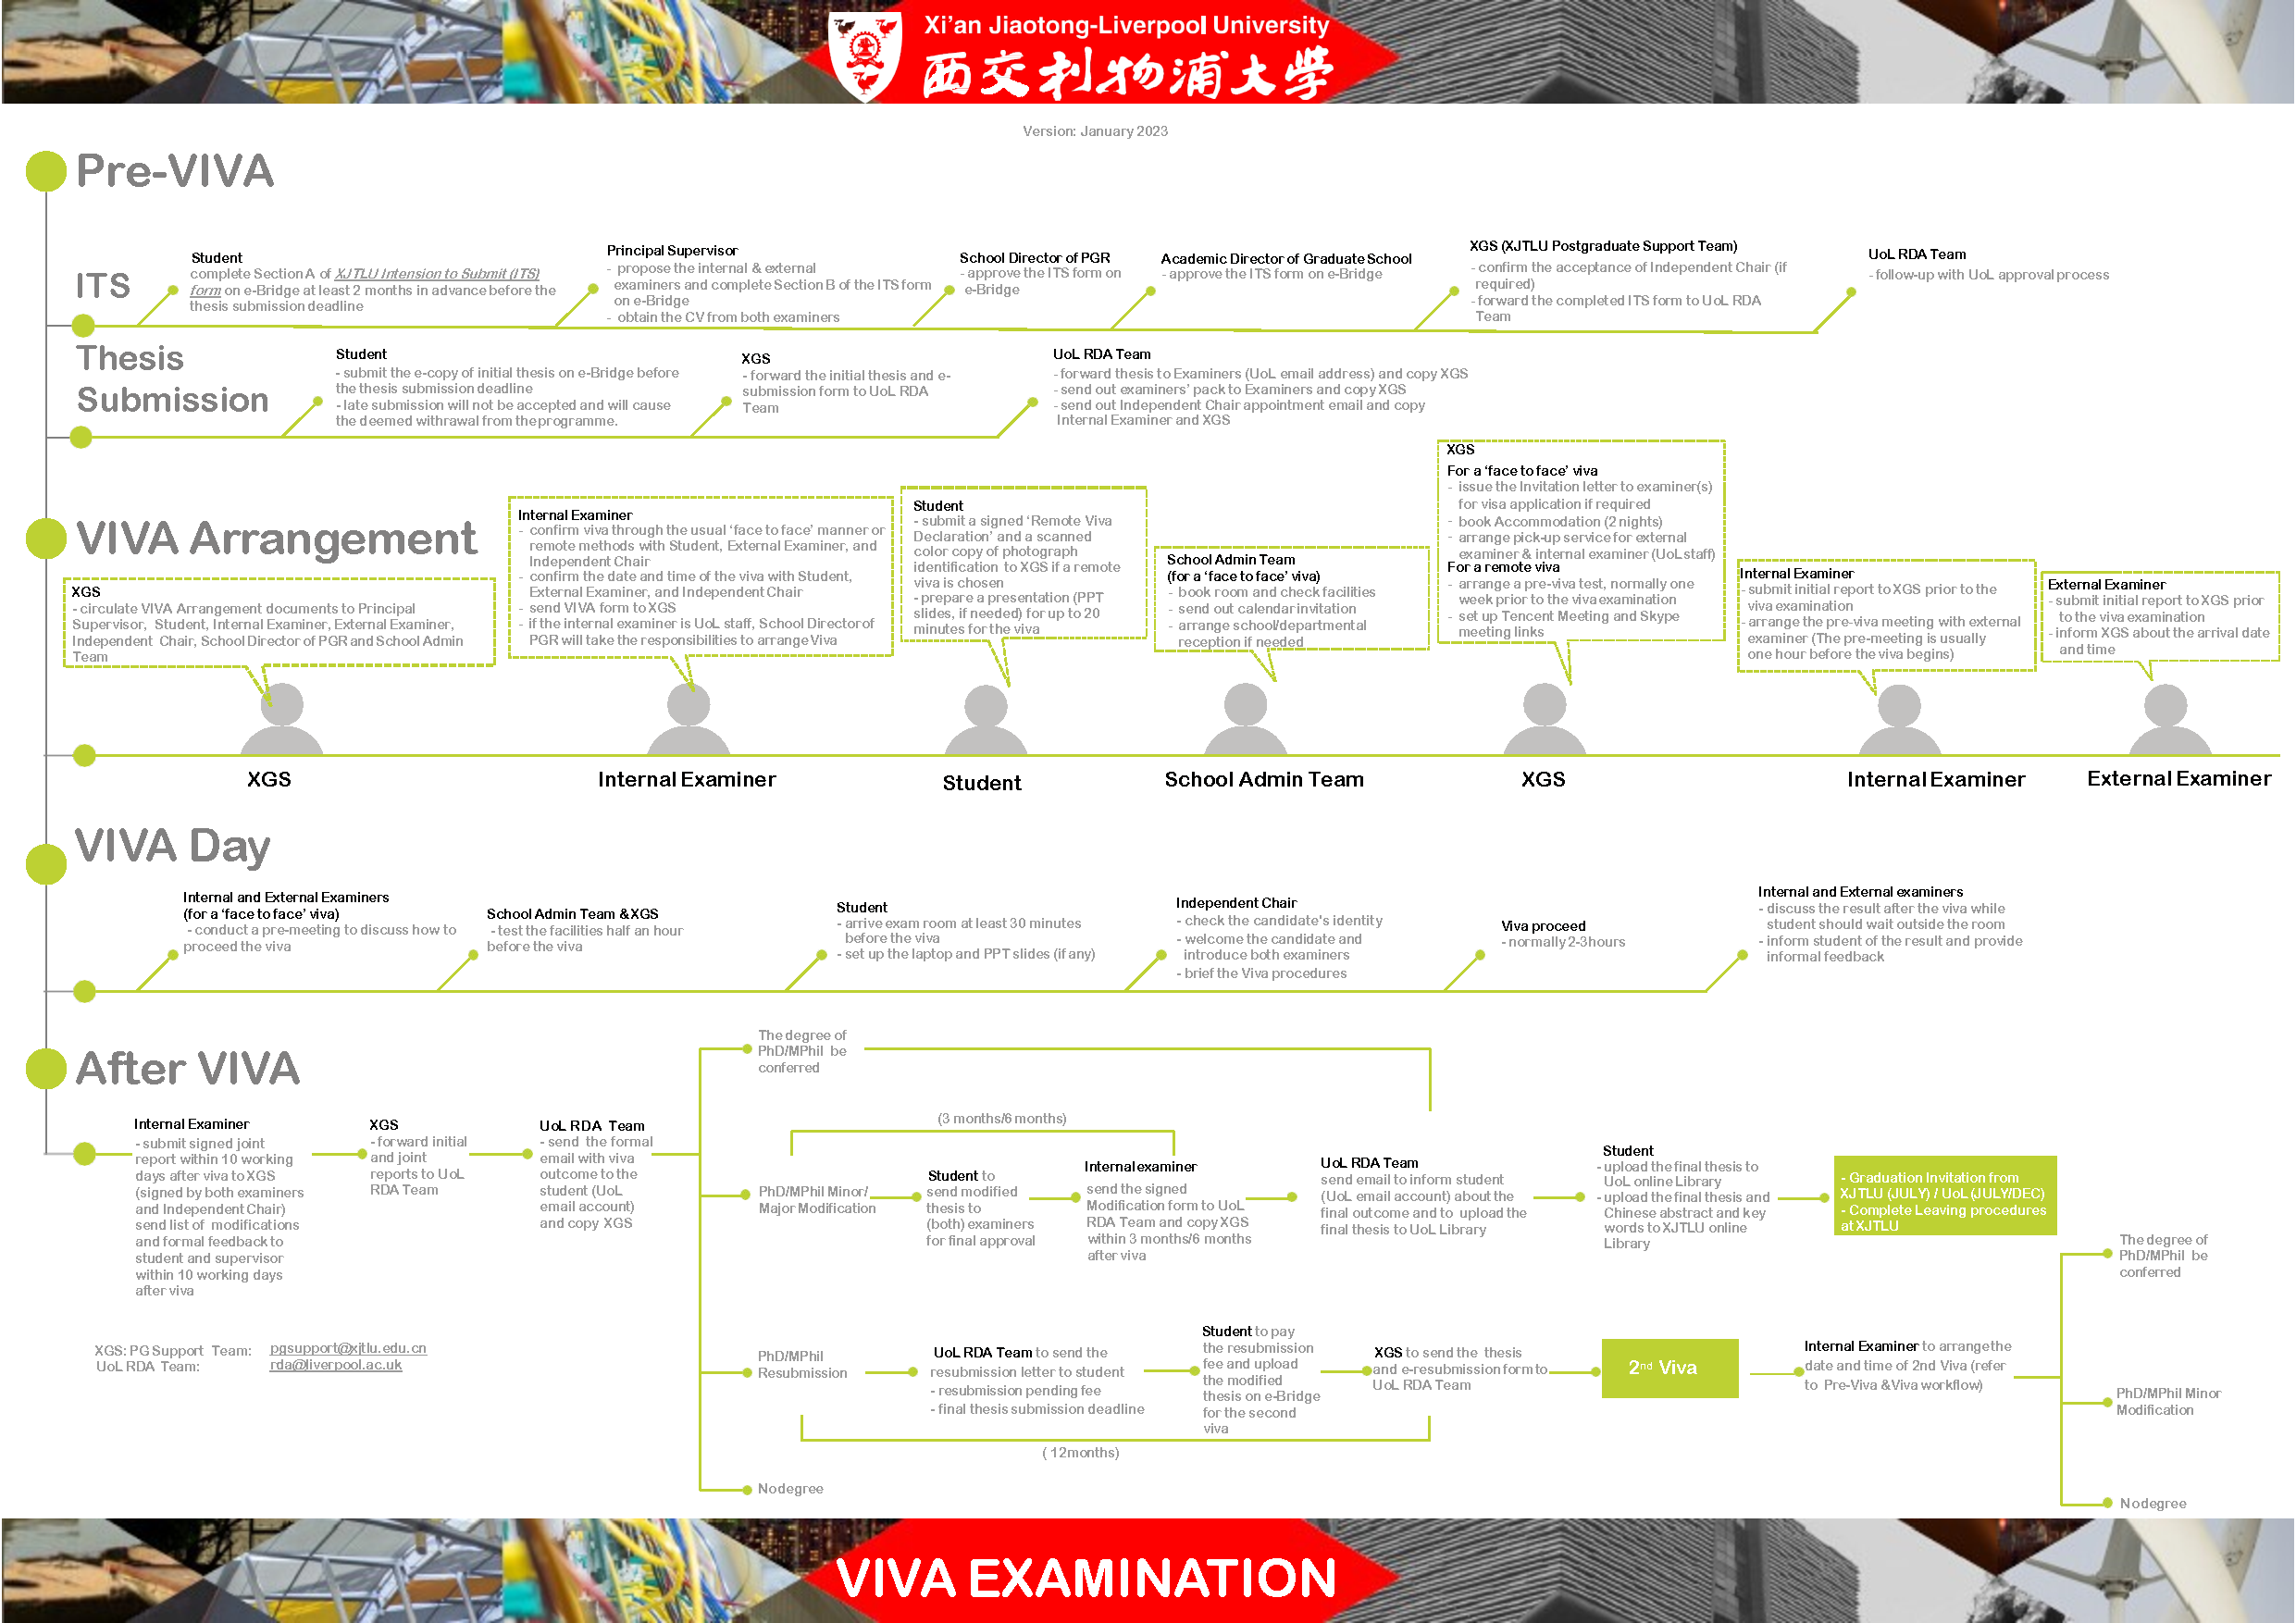
\includegraphics[width=\columnwidth]{fileshare/XJTLU VIVA Examination Arrangement Flowchart_2023.pdf}
    \caption{官方的毕业流程图。单独的文件可在fileshare里找到\url{https://gitee.com/kaiwu-astro/xp_pgrs_unofficial_guide/tree/main/fileshare}。注:我还真不知道这个文件在哪里下载的,这是我导发我的,想要最新版的可以在ebridge里找一下}
\end{figure}

如果想直到每个步骤大概要花多少时间,跳转章节 \ref{sec.graduation.time}。

\subsection{ITS: Intention to submit}

Q:ITS重要吗,我着急写论文呢,暂时不管它行不行

A:如果你对毕业时间有要求,请务必谨记尽早提交ITS表!ITS是你的论文和答辩一切程序的开始。现有规定,你的论文只能在\textbf{提交ITS之日起+2个月之后}才允许提交,可以延后,但不允许提前。(ITS提交后,一年内必须交论文;和你本身的论文deadline共同作用,以早的那个为准)

Q:ITS里面会填什么

A:毕业论文的题目、毕业论文的摘要、基本个人信息。题目和摘要不需要是最终决定的版本,也就是后面可以改。

Q:那我随便起个题目和摘要,走个过场行不行啊

A:这个表的作用是:导师和研究生院会拿着这个标题和摘要去决定你的内审、外审。这个题目和摘要也会发给他们。因此,和最终版可以有修改,但是也要尽量准确的反映你这几年的研究。

Q:我还要问

A:先看看官方文件:\url{https://www.liverpool.ac.uk/aqsd/academic-codes-of-practice/pgr-code-of-practice/}

\subsection{Thesis: 学位论文/毕业论文}

\subsubsection{格式和排版}

官方文件:\url{https://www.liverpool.ac.uk/media/livacuk/tqsd/code-of-practice-on-assessment/annex-7.1-PGR-CoP.pdf}
<-- 一切对格式不确定的请以这个为准。下面是微信群里的一些日经问题。

Q:可以用什么软件写毕业论文?

A:根据上面的规定,利物浦对软件没有要求,也就是你想用什么都可以。常用的有:Microsoft Word, \LaTeX

Q:推荐用什么软件呢

A:\LaTeX 优点:(1)非常方便输入公式,(2)参考文献和引用处理起来非常方便,不需要Endnote等外部软件辅助,(3)格式美观,风格统一,排版很难难看,(4)文件小,文件可分散,方便备份。\LaTeX 缺点:学习成本较高。如果你们专业发期刊论文/会议论文都不用\LaTeX 而用Word,那你切换过来就要花些时间学习。

Q:上面这个排版要求文件要求好多好细,呜呜呜给我一份毕业论文模板吧呜呜呜呜

A:
\begin{enumerate}
    \item Word还真的有一个官方模板,可以在本项目fileshare下载\url{https://gitee.com/kaiwu-astro/xp_pgrs_unofficial_guide/tree/main/fileshare}。来源:ELC Thesis Writing Camp的老师
    \item \LaTeX 没有官方模板,但数理学院(SMP)的大部分毕业生都是用\LaTeX 写的毕业论文。可以直接在Overleaf模板库直接搜索Liverpool Thesis,应该只有一个搜索结果,采用即可。
    \item 请使用模板的同学特别注意,never fully trust the template! Word模板是西浦ELC的老师给的,不是利物浦给的;Overleaf更是民间模板。理论上,他们对你的论文和毕业都\textbf{不负责}。因此拿到模板过后,第一件事永远还是打开上面的Code of Practice,一条一条的比对看是否达到了要求。
\end{enumerate}

\subsubsection{字数}

Q:上面的CoD只说了一个字数上限,那最低字数要求呢?

A:另一个日经问题。我曾经在研究生院Thesis Writing Camp课程上问了老师,他的意见是,西浦Master thesis的字数上限是3w,因此PhD thesis最好超过这个数。但我后来发现不是这回事。我见过有的论文不到100页,有的接近200页,都毕业了。从全校来看,这个是真的没有要求。你如果不放心,还是想对最低字数有点数,很简单,去利物浦图书馆和西浦图书馆下载毕业论文,重点参考你们学院、你们系、你们专业、最好直接是你同门已毕业同学的毕业论文,有多少字有多少页。\textbf{请谨记,字数多并不能保证你能轻松毕业}。我的一个师兄thesis就是接近200页,吃了个大改,外审说他写得太多了像教科书。

\begin{flushright}
    (2024年08月12日 by Kai Wu)
\end{flushright}

\subsection{论文答辩}

\subsubsection{答辩前后流程}

\begin{enumerate}
    \item 在e-bridge上正式提交论文之前至少两个月,由指导老师选定好未来答辩的考察老师名单,交由XJTLU的pgsupport以及利物浦审核确定。
    \item 在e-bridge上正式提交论文后,学校会联系对应的考察老师,之后再联系博士生候选人确定答辩时间以及答辩方式(答辩时间一般在提交论文的1-3个月内,答辩方式分为线上线下两种,具体可以跟pgsupport沟通确认)。
    \item 一般来说,答辩之前会有一次预演,可以用来测试网络以及ppt展示。也可以另外申请时间去对应的会议室讲演ppt。
    \item 答辩前,考察老师们会先内部开一个通气会,一般来说是当天(但也有提前时间的),然后再邀请你进入会议室正式开始答辩。除了两位(或三位(特殊规则下))考察老师外,还有一位观察老师(负责整体流程推进和休息安排,并回答你的流程相关问题,在正式答辩阶段,基本上不会说话),如果有任何问题,都可以问他。
    \item ppt讲完是问答流程,根据具体情况,时间在一个半到3个半小时是比较常见的情况(历史上也出现过7个小时的)。问答流程结束后会请你离开会议室一段时间,老师们进行结果讨论。大约10-15分钟后,请你进去并现场告知结果。
    \item 考察老师的修改意见报告会在10个工作日之内发给你,根据具体的情况你需要在规定的时间内进行修改并交由主审考察老师确认。
    \item 确认无误之后把最终版本的论文上传,这个流程就算是结束了。
\end{enumerate}

\begin{flushright}
    (2024年07月05日 by Ziwen Xie)
\end{flushright}


\subsubsection{如何准备好一场答辩}

来自理学院的经验:

\textit{尽量不要堆在两三天内做这些,把内容稍微分散一点,利于每天保持好状态,维持好状态进入正式答辩相当重要。}

\textbf{一. 至少完整的逐字逐句的读完自己的thesis一遍,假设自己是个全新读者,边读边思考下列问题}
\begin{enumerate}
    \item 某些段落会不会不够清楚
    \item 某些概念是否自己已经完全掌握能独立解释
    \item 章节与章节之间的联系与区别自己是否明白,以及整体文章排布顺序的内在逻辑
    \item 章节内部的小段落,实验设计顺序之间的内在逻辑
    \item 每个或者某几个实验能一起或者分别说明什么问题,每个大章节能总结出什么结论
    \item 具体引用的文献里的一些算法,一些模型,一些基础概念自己是否完全了解为什么是这样的。他们在文章中有什么关联性(与你的核心实验目标)
    \item 有没有之前没发现的表述错误或者图表错误(之后也需要改的)
    \item 你做这项研究的目的是什么,选择某种方法的动机是什么,比其他方法有什么优势
\end{enumerate}

\textbf{二. 整理好上述问题之后,一章章(abstract也含在内)的进行拆分来进行细节分析,包括:}
\begin{enumerate}
    \item 所有背景知识相关介绍的内容,自己能否用自己的话大概表述
    \item 每个小标题表达的内容是什么,整章节内的小标题统一性
    \item 具体实验的或者实验设计的亮点或者核心逻辑
    \item 具体实验结果之间的递进、并列或者其他关系和区别(比如A实验说明了a,B实验说明了b,a是进行实验B的逻辑基础,这就属于递进。如果a和b方向内容相同那就是A和B并列)
    \item 实验对象的选择和实验模型的选择的原因(也包括为啥不用别的相关或者类似的对象和模型)
    \item 基于获得的结果,还有什么是可以未来去尝试的(这个部分可以很多相关问题,包括为什么不做某些实验,未来做某些实验是为什么,未来做某些实验可能能得到什么,未来的某些实验的基础设想和实践难度(也就是为啥你现阶段没做,但是你考虑了))
    \item Abstract要包含关键的结果和创新点
\end{enumerate}

\textbf{三. 最后做ppt和viva的时候的相关重点}
\begin{enumerate}
    \item 一共二十分钟,可以分成四个部分(背景介绍,实验设定,实验结果,推断结论)。每个部分5分钟左右,尤其结尾部分,前面三个部分可以适当简短,毕竟考官都读过你的文章了。
    \item 打印好你的文章带去现场,边问答边做笔记(同时也给自己一些喘息时间(通过记笔记))
    \item 重点图表结果在ppt内展示,并附上简短的结论描述
    \item 不太需要讲遇到的问题,也不需要着重讲未来能做的实验或者设计(考官可能会问到,或者你回答某些问题的时候会答)根据具体情况,这部分可以放弃ppt部分讲,节约时间。
    \item 确保ppt能正常运行,字和图片都看得清,提前测试的时候,尽可能自己模拟实际讲的情况过一遍
    \item 答辩过程中记得喝水,但是慢慢喝,少量多次比较好。开始之前吃一些能量多好消化的食物,实在吃不下也吃点巧克力什么的或者弄点提神的饮品。开始之前多提前点到,熟悉环境有助于放平心态(也记得提前上厕所)
    \item 回答问题的时候可以横跨整个文章,有的章节内的点可能是在后续章节里有联动的,或者未来计划和最终结论相关的。如果遇到考官提出,自己确实没想到或者没做的,该说不知道就不知道,并且提出需求,希望考官在反馈部分明确相关信息的处理办法或者信息来源(方便你后续改的时候知道去哪找东西)。
    \item 一般来说每个问题的问答大概3-5分钟最多,两个考官的情况下,每个老师20个问题就算不少了。所以一般情况下是两个小时到两个半小时,中间会有休息时间的(不过等真的开始了,你应该不太会顾得上时间变化)。
\end{enumerate}
 
\textbf{四. 非论文相关问题}
\begin{enumerate}
    \item 人工智能和Chatgpt能如何inspire你的研究?
    \item 你的研究可以应用到其他类型的数据/疾病/领域吗?为什么?
    \item 你认为你的专业存在什么样的缺点?
    \item 你在读博几年中的最大收获是什么?
    \item 如果再来一次,你还会选择读博并做这个项目吗?
\end{enumerate}
Tips:感觉老师就是比较好奇聊聊,放松回答就行。\textbf{最后来源于PGsupport某老师的数据,咱们建校以来从未有过Fail的答辩结果,因此大家不要太担心,正常发挥就行,祝好运。} 

\textbf{五. 问问自己的老师能不能帮你设想一些问题,另外如果时间充裕,能不能让自己的老师给安排个模拟viva(可选项)。也鼓励去找自己的前辈们在他们答辩结束后去及时咨询相关情况,毕竟每年情况可能多少都会有一些变化。}

\begin{flushright}
    (2024年07月05日 by Ziwen Xie)
\end{flushright}


\subsection{我想尽快拿学位证!如何速通毕业流程}

急急急,你就是急急国王。下面是一个合格的急急国王必须知道的事。

\subsubsection{毕业的证明文件}

\begin{enumerate}
    \item 完读证明(Completion of Studies Certificate),由西浦研究生院开具。证明内容:已提交毕业论文,已通过答辩,即将在XXXX年X月的毕业典礼上授予博士学位。我的Example:
    \begin{figure}[H]
        \centering
        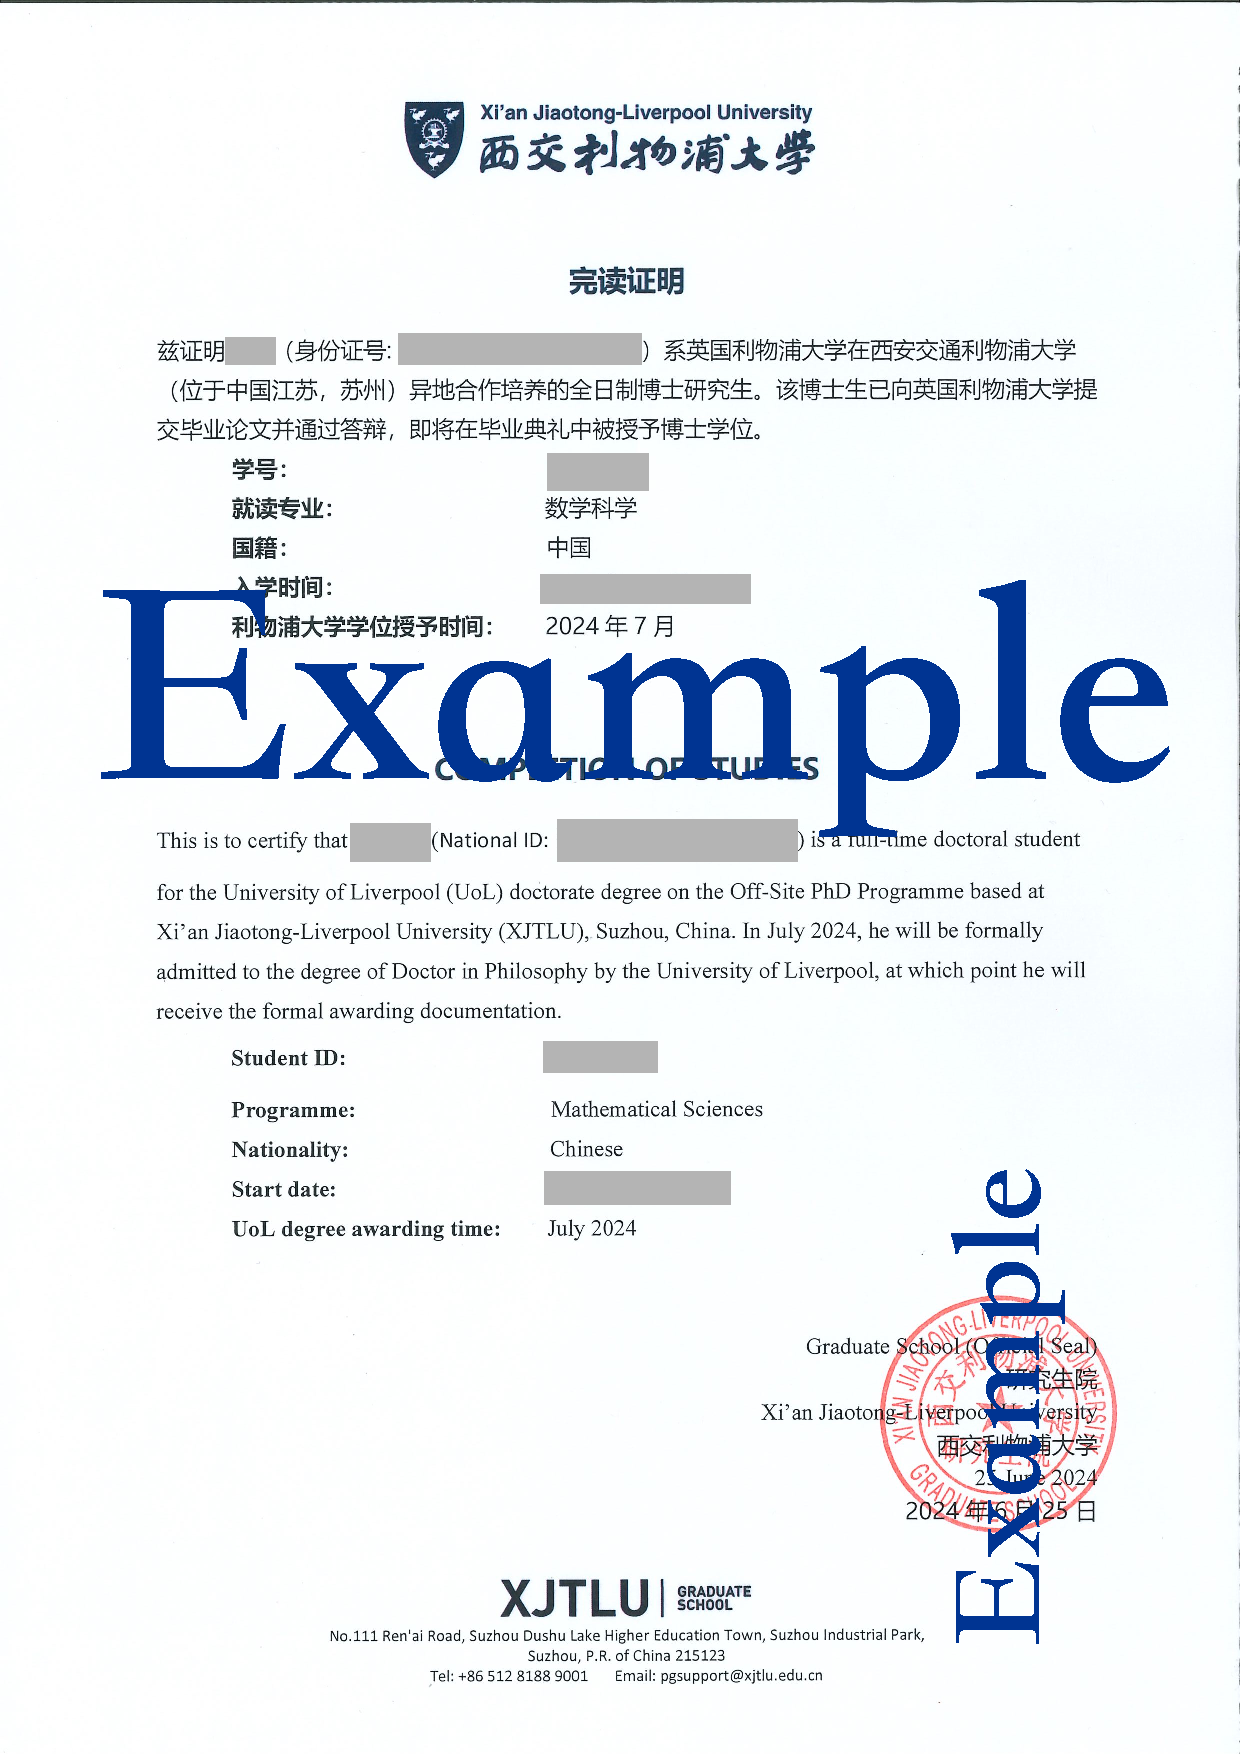
\includegraphics[width=0.8\columnwidth]{author-folder/Kai.Wu/Completion_of_Studies_Certificate_EXAMPLE.pdf}
        \caption{仅供参考,因此加上了巨大的example防止非法盗用}
    \end{figure}
    \item 学位证(aka PhD degree, degree certificate)。注意!利物浦规定,学位只会在\textbf{利物浦}毕业典礼上颁发,而利物浦毕业典礼一年只有两次,一般是7月某天和12月某天。如果你不去利物浦毕业典礼,会在毕业典礼前后先给学位证的电子版(有法律效力,可办中外合办认证),然后原件慢悠悠的邮寄到西浦。
    \item 中外合办学位认证。拿到电子学位证即可办理 \url{https://zwfw.cscse.edu.cn/}。持有该认证,你的利物浦学位就在中国境内被教育部承认。
\end{enumerate}

因此,首先确定你要去的公司/单位能接受哪种证明文件。最松的情况,你答辩完收到利物浦确认的Pass (with minor/major modification)邮件就行。也有能接受完读证明的。如果对方比较死板,不见学位证就不行,甚至没有中外合办认证也不行,那就要特别规划好毕业进度,因为每年只发2次证!

\subsubsection{学位证:最关键时间节点}

如果你确定不需要赶时间拿学位证,那本节接下来的都可以忽略,因为完读证明任何时候都可以开。

Q:我能否在7月/12月毕业?硬性要求是什么?

A:最好的方式是直接上利物浦网站查询,或者直接google liverpool phd graduation。过去几年的要求都是:在某个时间点之前,利物浦图书馆确认收到你的\sout{终极完全不改版的}最终论文。例如,如果要参加2024年7月15日的利物浦毕业典礼(在这一天颁发学位证,或邮寄),需要在2024年6月25日之前,利物浦图书馆确定收到了最终论文。这份论文是你的内外审都满意、同意的最终版。如何走到这一步?看下一节。

\subsubsection{每个步骤要等多久?如何预估时间?}
\label{sec.graduation.time}

以下完全基于已毕业同学的经验整理。新毕业的同学,请不吝赐教,补充你的真实案例。

以 \ref{sec.official.flowchart} 中提到的流程图来梳理:
\begin{enumerate}
    \item ITS:你提交过后其实就不用管了,专心写论文吧,剩下的都是导师和研究生院的活。背后的流程:i. 导师propose内审老师、外审老师; ii.研究生院审核,可能因为觉得这个老师和你利益相关等原因驳回其中的某人,然后你导师重新propose,直到研究生院满意为止,定下来内审外审人选各一个。在这个阶段,严格来说你直到论文提交都不能直到内外审老师是谁,导师需要保密,所以也不要\textbf{太}为难你导师去问是谁。
    \item 首次论文提交 到 论文答辩:(30天±30天)提交后,西浦研究生院(XGS)和利物浦学位办(RDA)会花两三个工作日简单处理下论文,发给内外审。\textbf{内审}一旦收到论文,就负责安排答辩时间。也就是说,你的答辩日期完全取决于你+内审+外审+独立主席(independent chair)都有空的某个时候(正常2-3小时)。因此,最早答辩日 = 论文交了过后三四个工作日;最晚答辩日则没有规定,找到四个人有空的时间为止。如果你赶时间,你能做的:(1)论文提交过后,尽早找你的内审,催ta安排日期;(2)把你论文提交过后一两个月的日程尽量腾空,不要因为自己的日程耽误答辩;(3)内外审一旦决定就不好更换,但独立主席容易换(有时会出现答辩一周前主席没空,找人另一老师顶上的事情),如果你们四个人里面是主席时间不合适导致拖很晚,尽早找你导师看能不能换主席。正常来说:交论文+60天=答辩 算非常慢的(但也有例子,据说是交论文前后不巧遇到了利物浦搞罢工)。一般会在+30天左右。
    \item 答辩完成 到 最终论文通过:(0 - 180天,典型为3-4周)。根据答辩结果不同这一步会有很大区别。(1) Pass (无条件) = 0天,论文初版即为最终版。(2) Pass with minor modification (小改),绝大部分同学都是这个结果。(3)Pass with major mofication(大改)(其他比较惨的情况很少,\sout{建议让导师和他举荐的examiner打一架})。如果是2或3,内外审会在10工作日(=2周)内出具书面的修改报告。这个过程个人建议不要催,他们要交的表和报告不少。之后就取决于你能多快改完论文。改完过后,按利物浦邮件指示,把改好的论文用指定的方式发给老师。这一步完全取决于你的内外审老师多久能respond,以及他们对你的修改是否满意。因为按照流程,如果不满意,他们有权让你改到他们满意为止。为了避免反复迭代,建议和导师反复斟酌新文本,争取一次搞定。这个版本的论文不会自动作为最终版,你可以在里面用颜色或者加粗标注修改过的地方,方便两位老师查阅。
    \item 最终论文通过 到 利物浦图书馆确认收到:(7天)这一步只是行政手续。在通过后,RDA会发邮件通知你上传最终论文(我的情况:内审老师告诉我[他们已告诉XGS和RDA修改版通过],过了4天收到上传通知),然后你将最终论文发送给利物浦,过几天(我的情况:2天)就收到利物浦图书馆正式通知邮件,论文成功上传。
    \item 实际还有一些手续,比如西浦会也让你上传一份到西浦图书馆,不知道是否会影响毕业,收到通知过后也最好尽早完成。
    \item 电子degree:具有法律效力的电子版degree会在你毕业典礼日期的前后几天内颁发。按照利物浦给你的邮件,在verify.liverpool.ac.uk里查询。
    \item 纸质degree:如果你人去利物浦参加毕业典礼,那就是现场领取。如果你不去,会在你毕业典礼日期后官方邮寄到西浦,等就完事了。我的情况:7月15日利物浦毕业典礼(人没去),纸质版7月30日寄到了研究生院。如果到时候人已经不在学校,可以委托研究生院邮寄(不推荐,丢件没法补,风险自担)。
\end{enumerate}

\begin{flushright}
    (2024年08月12日 by Kai Wu)
\end{flushright}